\documentclass[pdflatex,compress]{beamer}

%\usetheme[dark,framenumber,totalframenumber]{ElektroITK}
\usetheme[darktitle,framenumber,totalframenumber]{ElektroITK}
\usepackage{graphicx}
\usepackage{multicol}

\title{Data Communications}
\subtitle{Chapter 6 - Error Detection and Correction}

\author{Mifta Nur Farid}

\begin{document}

\maketitle

\begin{frame}
	\frametitle{Types of Errors}
	\begin{itemize}
		\item An error occurs when a bit is altered between transmission and reception
		\begin{itemize}
			\item Binary 1 is transmitted and binary 0 is received
			\item Binary 0 is transmitted and binary 1 is received
		\end{itemize}
		\item \textbf{Single bit errors}
		\begin{itemize}
			\item Isolated error that alters one bit but does not affect nearby bits
			\item Can occur in the presence of white noise
		\end{itemize}
		\item \textbf{Burst errors}
		\begin{itemize}
			\item Contiguous sequence of B bits in which the first and last bits and any number of intermediate bits are received in error
			\item Can be caused by impulse noise or by fading in a mobile wireless environment
			\item Effects of burst errors are greater at higher data rates
		\end{itemize}
	\end{itemize}
\end{frame}

\begin{frame}
	\frametitle{Burst and Single-Bit Errors}
	\begin{center}
		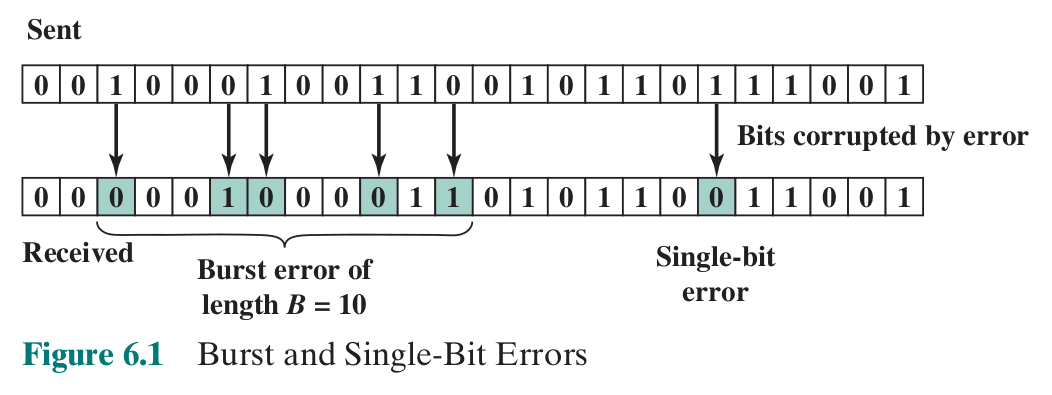
\includegraphics[width=\linewidth]{img/img01}
	\end{center}
\end{frame}

\begin{frame}
	\frametitle{Error Detection}
	\begin{itemize}
		\item Regardless of design you will have errors, resulting in the change of one or more bits in a transmitted frame
		\item Frames
		\begin{itemize}
			\item Data transmitted as one or more contiguous sequences of bits
			\item[$ P_b $ :] Probability that a bit is received in error; also known as the bit error rate (BER)
			\item[$ P_1 $ :] Probability that a frame arrives with no bit errors
			\item[$ P_2 $ :] Probability that, with an error-detecting algorithm in use, a frame arrives with one or more undetected errors
			\item[$ P_3 $ :] Probability that, with an error-detecting algorithm in use, a frame arrives with one or more detected bit errors but no undetected bit errors
		\end{itemize}
	\end{itemize}
\end{frame}

\begin{frame}{Error Detection}
	\begin{itemize}
		\item The probability that a frame arrives with no bit errors decreases when the probability of a single bit error increases
		\item The probability that a frame arrives with no bit errors decreases with increasing frame length
		\begin{itemize}
			\item The longer the frame, the more bits it has and the higher the probability that one of these is in error
		\end{itemize}
	\end{itemize}
\end{frame}

\begin{frame}
	\frametitle{Error Detection Process}
	\begin{center}
		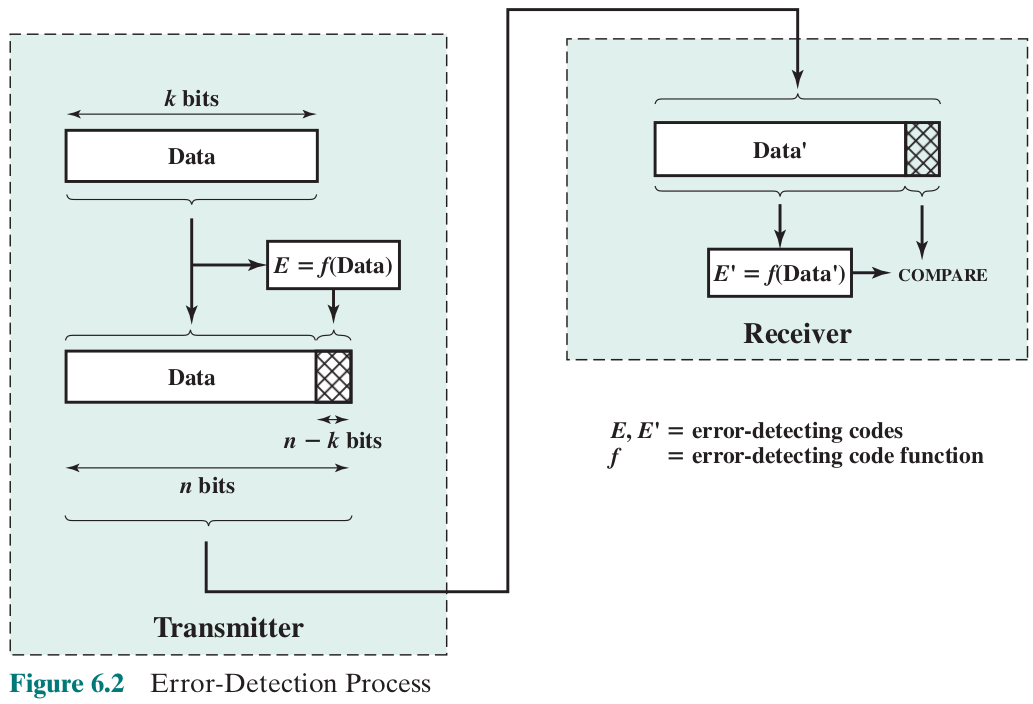
\includegraphics[width=\linewidth]{img/img02}
	\end{center}
\end{frame}

\begin{frame}
	\frametitle{Parity Check}
	\begin{itemize}
		\item The simplest error detecting scheme is to append a parity bit to the end of a block of data
		\begin{itemize}
			\item Even Parity
			\begin{itemize}
				\item Even number of 1s
				\item Used for synchronous transmission
			\end{itemize}
			\item Odd Parity
			\begin{itemize}
				\item Odd number of 1s
				\item Used for asynchronous transmission
			\end{itemize}
		\end{itemize}
		\item If any even number of bits are inverted due to error, an undetected error occurs
	\end{itemize}
\end{frame}

\begin{frame}
	\frametitle{A Two-Dimensional Even Parity Scheme}
	\begin{center}
		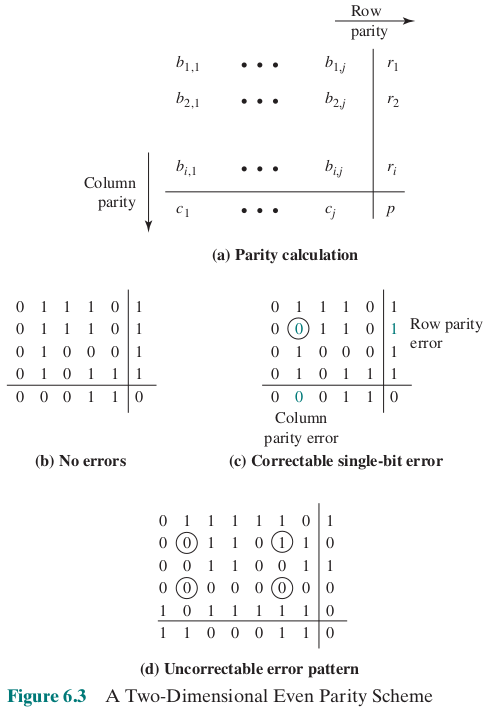
\includegraphics[height=0.8\textheight]{img/img03}
	\end{center}
\end{frame}

\begin{frame}
	\frametitle{The Internet Checksum}
	\begin{itemize}
		\item Error detecting code used in many Internet standard protocols, including IP, TCP, and UDP
		\item Ones-complement operation
		\begin{itemize}
			\item Replace 0 digits with 1 digits and 1 digits with 0 digits
		\end{itemize}
		\item Ones-complement addition
		\begin{itemize}
			\item The two numbers are treated as unsigned binary integers and added
			\item If there is a carry out of the leftmost bit, add 1 to the sum (end-around carry)
		\end{itemize}
	\end{itemize}
\end{frame}

\begin{frame}
	\frametitle{Example of Internet Checksum}
	\begin{center}
		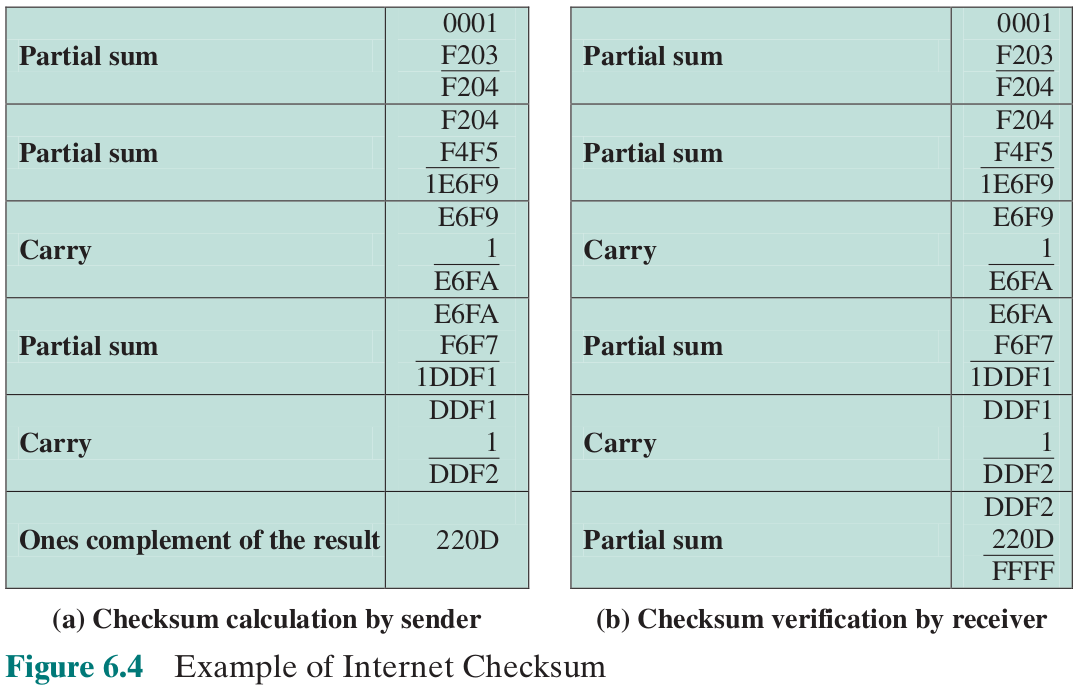
\includegraphics[width=\linewidth]{img/img04}
	\end{center}
\end{frame}

\begin{frame}
	\frametitle{Cyclic Redundancy Check}
	\begin{itemize}
		\item one of most common and powerful checks
		\item for a block of k bits transmitter generates an n bit frame check sequence (FCS)
		\item transmits k+n bits which is exactly divisible by some number
		\item receiver divides frame by that number
		\begin{itemize}
			\item if no remainder, assume no error
			\item for math, see Chapter 6
		\end{itemize}
	\end{itemize}
\end{frame}

\begin{frame}
	\frametitle{CRC Process}
	\begin{itemize}
		\item Modulo 2 arithmetic
		\begin{itemize}
			\item Uses binary addition with no carries
			\item An example is shown on page 218 in the textbook
		\end{itemize}
		\item Polynomials
		\begin{itemize}
			\item Express all values as polynomials
			in a dummy variable X, with
			binary coefficients
			\item Coefficients correspond to the bits in the binary number
			\item An example is shown on page 221 in the textbook
		\end{itemize}
	\end{itemize}
\end{frame}

\begin{frame}{CRC Process}
	\begin{itemize}
		\item Digital logic
		\begin{itemize}
			\item Dividing circuit consisting of XOR gates and a shift register
			\item Shift register is a string of 1-bit storage devices
			\item Each device has an output line, which indicates the value currently stored, and an input line
			\item At discrete time instants, known as clock times, the value in the storage device is replaced by the value indicated by its input line
			\item The entire register is clocked simultaneously, causing a 1-bit shift along the entire register
			\item An example is referenced on page 223 in the textbook
		\end{itemize}
	\end{itemize}
\end{frame}

\begin{frame}
	\frametitle{Modulo 2 Arithmetic (XOR)}
	\begin{itemize}
		\item Define:
		\begin{itemize}
			\item $ T = n $-bit frame to be transmitted, $ n < k $
			\item $ D = k $-bit block data, or message, the first $ k $ bits of $ T $
			\item $ F = (n-k) $-bit FCS, the last $ (n-k)$ bits of $ T $
			\item $ P = $ pattern of $ n-k+1 $ bits, the predetermined divisor
		\end{itemize}
		\item We would like T/P to have no remainder
		\begin{itemize}
			\item $ T=2^{n-k} D+F $
			\item $ 2^{n-k} D/P = Q + R/P $, $ R $ is at least one bit less than $ P $
			\item Use $ R $ as the FCS (i.e. $ F $), i.e. $ T = 2^{n-k}D + R $
			\item Examine if $ T/P $ have no remainder?
			\begin{itemize}
				\item $ T/P = (2^{n-k}D + R)/P = Q + R/P + R/P = Q + (R+R)/P = Q $
			\end{itemize}
		\end{itemize}
	\end{itemize}
\end{frame}

\begin{frame}{Modulo 2 Arithmetic (XOR)}
	\begin{itemize}
		\item Occurrence of errors
		\begin{itemize}
			\item $ T_r = T + E $
			\item $ T = $ transmitted frame
			\item $ E = $ error pattern with 1s in positions of error
			\item $ T_r = $ received frame
		\end{itemize}
		\item Fail to detect an error if and only if $ T_r $ is divisible by $ P $
		\begin{itemize}
			\item i.e. if and only if $ E $ is divisible by $ P $
		\end{itemize}
	\end{itemize}
\end{frame}

\begin{frame}
	\begin{center}
		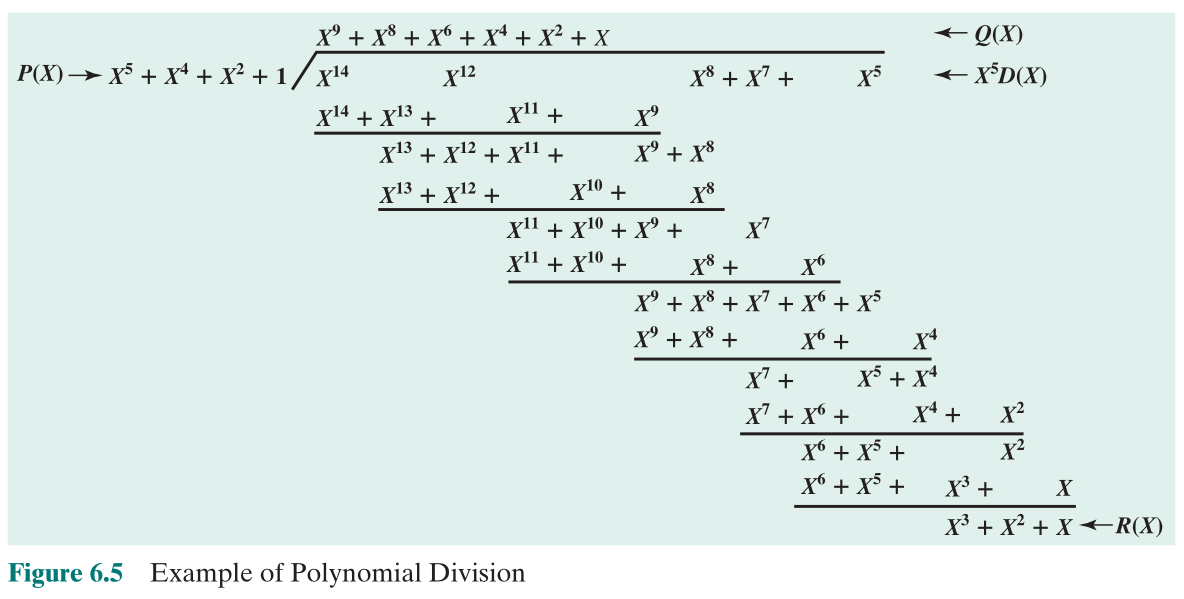
\includegraphics[width=\linewidth]{img/img05}
	\end{center}
\end{frame}

\begin{frame}
	\begin{center}
		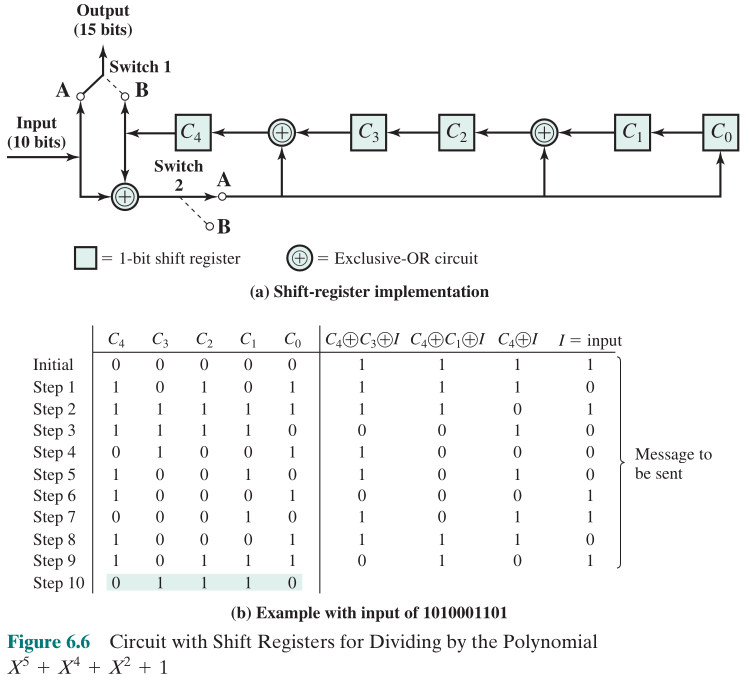
\includegraphics[width=0.7\linewidth]{img/img06}
	\end{center}
\end{frame}

\begin{frame}
	\begin{center}
		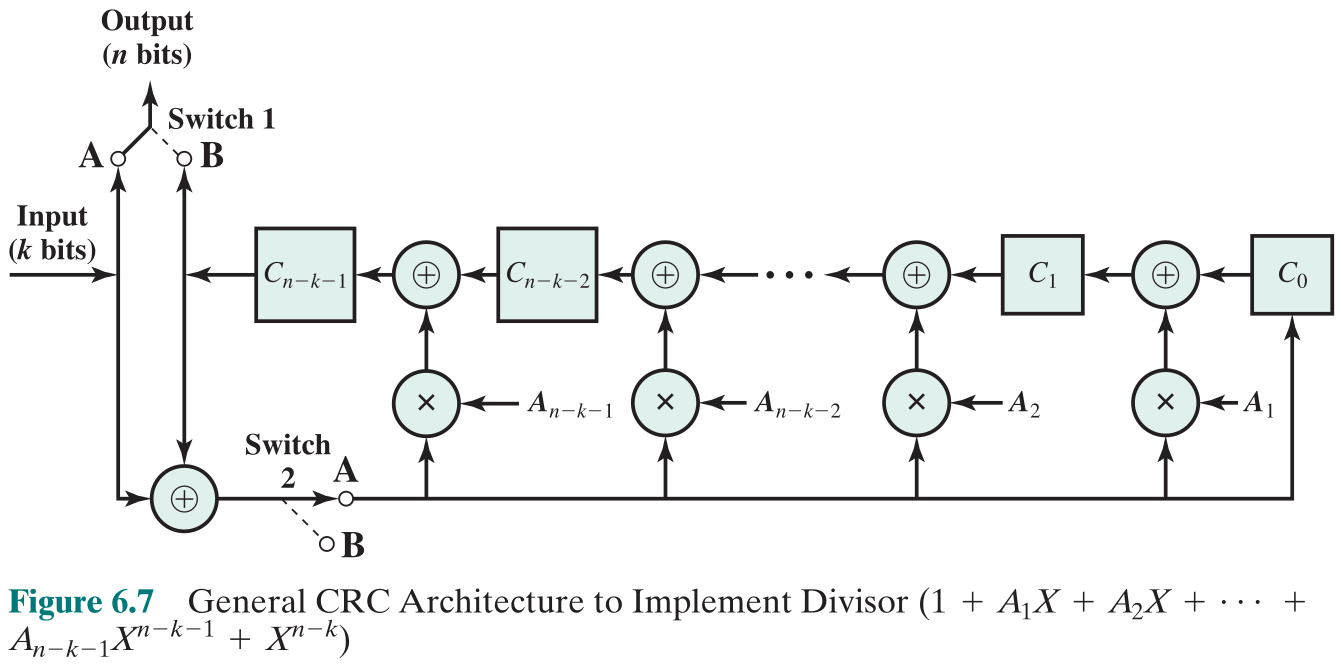
\includegraphics[width=\linewidth]{img/img07}
	\end{center}
\end{frame}

\begin{frame}
	\frametitle{Forward Error Correction}
	\begin{itemize}
		\item Correction of detected errors usually requires data blocks to be retransmitted
		\item Not appropriate for wireless applications:
		\begin{itemize}
			\item The bit error rate (BER) on a wireless link can be quite high, which would result in a large number of retransmissions
			\item Propagation delay is very long compared to the transmission time of a single frame
		\end{itemize}
		\item Need to correct errors on basis of bits received
		\item Codeword
		\begin{itemize}
			\item On the transmission end each k-bit block of data is mapped into an $ n $-bit block ($ n > k $) using a forward error correction (FEC) encode
		\end{itemize}
	\end{itemize}	
\end{frame}

\begin{frame}
	\begin{center}
		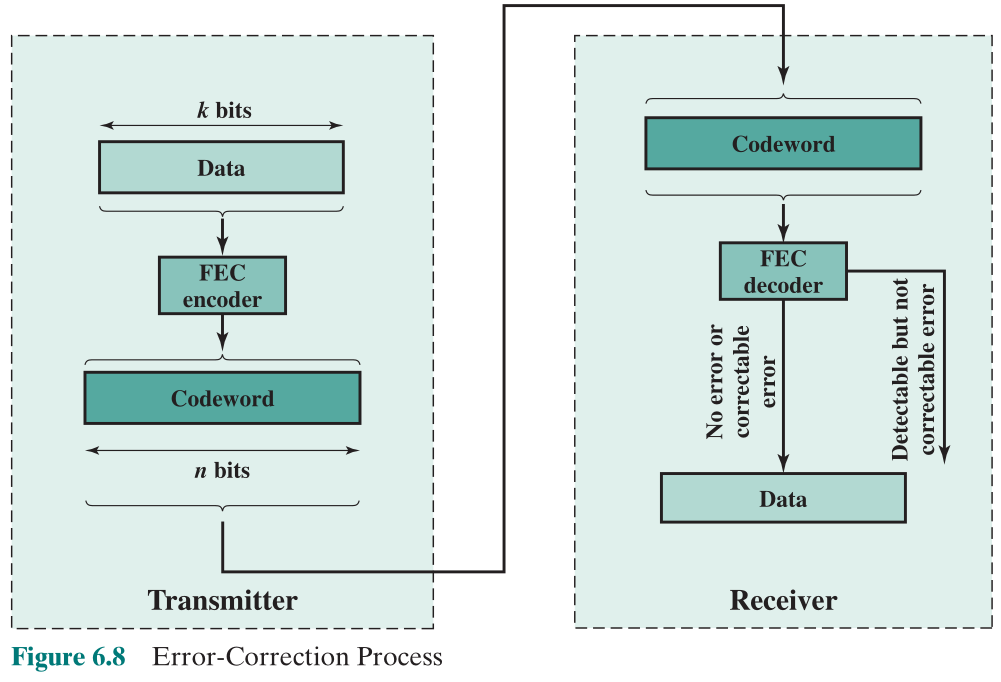
\includegraphics[width=\linewidth]{img/img08}
	\end{center}
\end{frame}

\begin{frame}
	\frametitle{Block Code Principles}
	\begin{itemize}
		\item Hamming distance
		\begin{itemize}
			\item $ d(v_1, v_2) $ between two $ n $-bit binary sequences $ v_1 $ and $ v_2 $ is the number of bits in which $ v_1 $ and $ v_2 $ disagree
			\item See example on page 227 in the textbook
		\end{itemize}
		\item Redundancy of the code
		\begin{itemize}
			\item The ratio of redundant bits to data bits $ (n-k)/k $
		\end{itemize}
		\item Code rate
		\begin{itemize}
			\item The ratio of data bits to total bits $ k/n $
			\item Is a measure of how much additional bandwidth is required to carry data at the same data rate as without the code
			\item See example on page 229 in the textbook
		\end{itemize}
	\end{itemize}
\end{frame}

\begin{frame}
	\begin{center}
		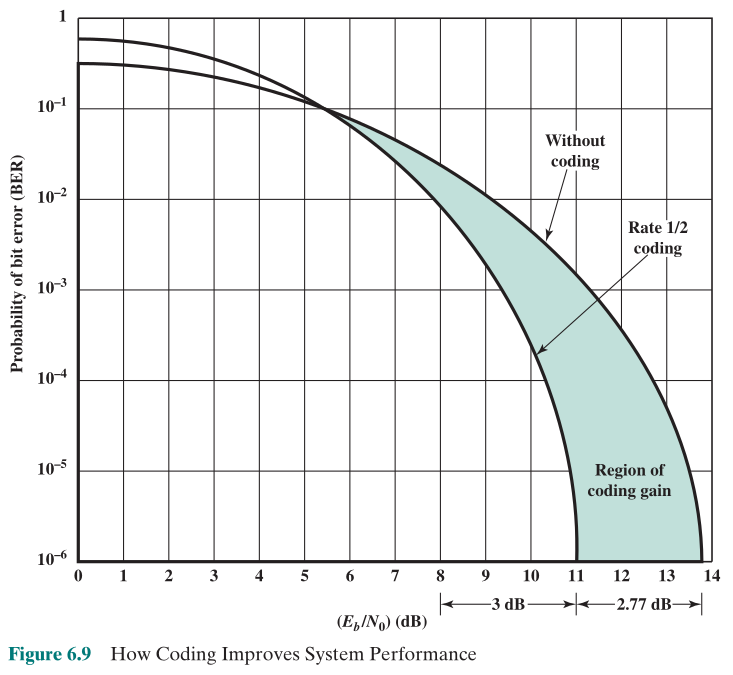
\includegraphics[width=0.7\linewidth]{img/img09}
	\end{center}
\end{frame}

\begin{frame}
	\frametitle{Summary}
	\begin{multicols}{2}
	\begin{itemize}
		\item Types of errors
		\item Error detection
		\item Parity check
		\begin{itemize}
			\item Parity bit
			\item Two-dimensional parity check
		\end{itemize}
		\item Internet checksum
		\item Cyclic redundancy check
		\begin{itemize}
			\item Modulo 2 arithmetic
			\item Polynomials
			\item Digital logic
		\end{itemize}
		\item Forward error correction
		\begin{itemize}
			\item Block code principles
		\end{itemize}
	\end{itemize}
	\end{multicols}
\end{frame}

\begin{frame}
	\frametitle{Tugas Mandiri}
	\begin{itemize}
		\item Stallings, W. (2014). Data and Computer Communications, 10th Edition, New Jersey: Upper Saddle River
		\begin{itemize}
			\item Chapter 6 Error Detection and Correction
		\end{itemize}
		\item Gupta, P. C. (2006). Data Communications and Computer Networks. New Delhi: Prentice Hall of India
		\begin{itemize}
			\item Chapter 5 Error Control
		\end{itemize}
		\item Tanenbaum, A. S. \& Wetherall, D. J. (2013). Computer Networks, Fifth Edition. London: Pearson.
		\begin{itemize}
			\item Section 3.2 Error Detection and Correction
		\end{itemize}
	\end{itemize}
\end{frame}

\begin{frame}
	\frametitle{Tugas Terstruktur}
	\textbf{Tampilkan Tugas 5}
\end{frame}

\end{document}
